\usetikzlibrary{fit, calc, positioning, arrows.meta}

\chapter{Strutture dati per insiemi disgiunti}

\section{A cosa servono}
\begin{itemize}
    \item Utili per la programmazione Greedy
    \item Alcune applicazioni richiedono
    \begin{itemize}
        \item Di raggruppare $n$ elementi distinti in una collezione di insiemi disgiunti
        \item L'esecuzione di 2 particolari operazioni
        \begin{itemize}
            \item Trovare l'(unico) insieme al quale appartiene un qualunque dato elemento
            \item Unire due insiemi
        \end{itemize}
    \end{itemize}
\end{itemize}

\section{Definizione}
Sia $X = \{x_1, \dots, x_n\}$ un insieme di $n$ elementi una struttura dati per insiemi (dinamici, essendo che variano nel tempo) disgiunti rappresenta / mantiene una collezione $\{S^1, \dots, S^k\} \text{ con $k \leq n$}$

\begin{figure}[htbp]
\centering
    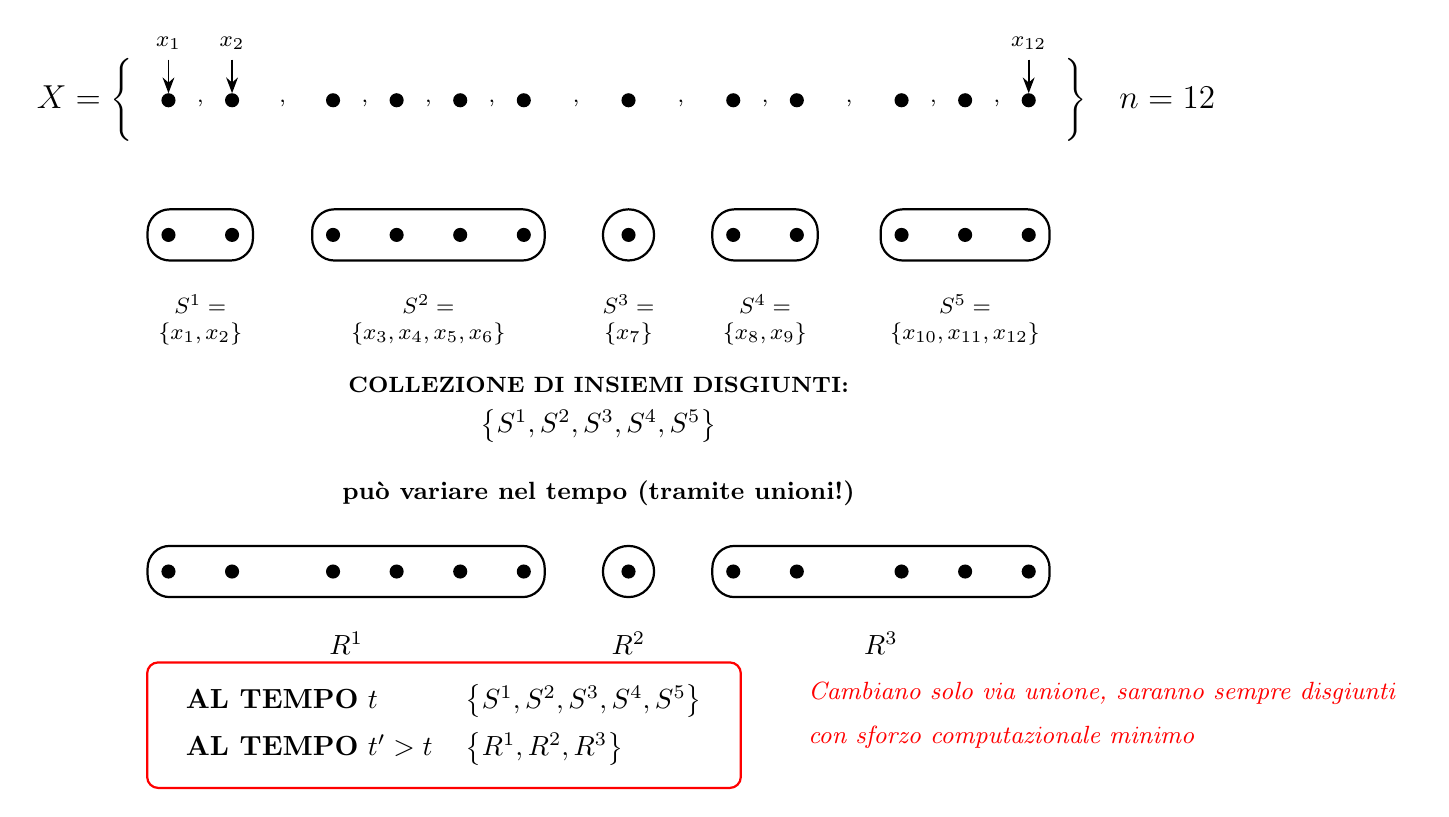
\begin{tikzpicture}[
        scale=0.95,
        dot/.style = {circle, fill=black, inner sep=1.8pt, outer sep=0pt},
        setbox/.style = {draw=black, thick, rounded corners=8pt, minimum height=0.65cm, inner xsep=5pt, inner ysep=2pt},
        singlebox/.style = {draw=black, thick, circle, minimum size=0.65cm, inner sep=0pt},
        arr/.style = {-{Stealth[length=2mm]}, semithick}
    ]

        % Coordinate orizzontali dei 12 punti, raggruppati per spaziare le etichette
        \def\xlist{0.0, 0.85, 2.2, 3.05, 3.9, 4.75, 6.15, 7.55, 8.4, 9.8, 10.65, 11.5}

        % =========================================================
        % 1. LIVELLO SUPERIORE: INSIEME X (n = 12)
        % =========================================================
        \foreach \x [count=\i] in \xlist {
            \node[dot] (x\i) at (\x, 0) {};
        }

        % Frecce ed etichette per gli elementi notevoli
        \draw[arr] (x1.north) ++(0, 0.45) node[above, font=\footnotesize] {$x_1$} -- (x1.north);
        \draw[arr] (x2.north) ++(0, 0.45) node[above, font=\footnotesize] {$x_2$} -- (x2.north);
        \draw[arr] (x12.north) ++(0, 0.45) node[above, font=\footnotesize] {$x_{12}$} -- (x12.north);

        % Virgole collocate a metà tra i nodi
        \foreach \i [evaluate=\i as \next using int(\i+1)] in {1,...,11} {
            \path (x\i) -- (x\next) node[midway, font=\footnotesize, yshift=-1pt] {,};
        }

        % Parentesi e dichiarazione insieme X
        \node[anchor=east, font=\large] at (-0.35, 0) {$X = \Bigg\{$};
        \node[anchor=west, font=\large] at (11.85, 0) {$\Bigg\} \quad \normalsize n = 12$};

        % =========================================================
        % 2. LIVELLO MEDIO: PARTIZIONE AL TEMPO t (INSIEMI S)
        % =========================================================
        \foreach \x [count=\i] in \xlist {
            \node[dot] (s\i) at (\x, -1.8) {};
        }

        % Raggruppamenti (capsule e cerchi)
        \node[setbox, fit=(s1) (s2)]   (boxS1) {};
        \node[setbox, fit=(s3) (s6)]   (boxS2) {};
        \node[singlebox, fit=(s7)]     (boxS3) {};
        \node[setbox, fit=(s8) (s9)]   (boxS4) {};
        \node[setbox, fit=(s10) (s12)] (boxS5) {};

        % Etichette insiemi S
        \node[below=3mm of boxS1, align=center, font=\footnotesize] {$S^1 =$\\$\{x_1, x_2\}$};
        \node[below=3mm of boxS2, align=center, font=\footnotesize] {$S^2 =$\\$\{x_3, x_4, x_5, x_6\}$};
        \node[below=3mm of boxS3, align=center, font=\footnotesize] {$S^3 =$\\$\{x_7\}$};
        \node[below=3mm of boxS4, align=center, font=\footnotesize] {$S^4 =$\\$\{x_8, x_9\}$};
        \node[below=3mm of boxS5, align=center, font=\footnotesize] {$S^5 =$\\$\{x_{10}, x_{11}, x_{12}\}$};

        % =========================================================
        % 3. TESTI DI SEPARAZIONE E TRANSIZIONE TEMPORALE
        % =========================================================
        \node[font=\footnotesize\bfseries] at (5.75, -3.8) {COLLEZIONE DI INSIEMI DISGIUNTI:};
        \node[font=\normalsize]           at (5.75, -4.35) {$\bigl\{ S^1, S^2, S^3, S^4, S^5 \bigr\}$};
        \node[font=\small\bfseries]        at (5.75, -5.25) {può variare nel tempo (tramite unioni!)};

        % =========================================================
        % 4. LIVELLO INFERIORE: PARTIZIONE AL TEMPO t' > t (INSIEMI R)
        % =========================================================
        \foreach \x [count=\i] in \xlist {
            \node[dot] (r\i) at (\x, -6.3) {};
        }

        % Raggruppamenti dopo unioni
        \node[setbox, fit=(r1) (r6)]   (boxR1) {};
        \node[singlebox, fit=(r7)]     (boxR2) {};
        \node[setbox, fit=(r8) (r12)] (boxR3) {};

        % Etichette insiemi R
        \node[below=3mm of boxR1, font=\normalsize] {$R^1$};
        \node[below=3mm of boxR2, font=\normalsize] {$R^2$};
        \node[below=3mm of boxR3, font=\normalsize] {$R^3$};

        % =========================================================
        % 5. RIEPILOGO STATI TEMPORALI
        % =========================================================
        % Box rosso grande che contiene il testo
        \node[anchor=north west, draw=red, thick, rounded corners=4pt, inner sep=8pt] at (-0.3, -7.5) {
            \begin{tabular}{ll}
                \textbf{AL TEMPO} $t$       & $\bigl\{ S^1, S^2, S^3, S^4, S^5 \bigr\}$ \\[1.2ex]
                \textbf{AL TEMPO} $t' > t$  & $\bigl\{ R^1, R^2, R^3 \bigr\}$
            \end{tabular}
        };
        \node[anchor=north west, font=\small\itshape, text=red] at (8.2, -7.6) {
        \begin{tabular}{l}
            Cambiano solo via unione, saranno sempre disgiunti \\[1.2ex]
            con sforzo computazionale minimo
        \end{tabular}
        };
    \end{tikzpicture}
\caption*{Rappresentazione grafica}
\end{figure}

\newpage
\section{Proprietà degli insiemi disgiunti}
    \begin{itemize}
        \item $\forall i \in \{1, \dots, k\}, \quad S^i \subseteq X$ \\ Ogni elemento appartiene ad un insieme
        \item $\forall i,j \in \{1, \dots, k\} \text{ con $i \not = j$} \quad S^i \cap S^j = \emptyset$\\ Non abbiamo elementi condivisi tra insiemi
        \item $\bigcup_{i=1}^{k} S^i = X$\\ L'unione di tutto gli insiemi disgiunti risulta nella costruzione dell'insieme originario X
        \item La collezione può variare nel tempo, ma essa continuerà sempre una partizione di $X$
        \item Ciascun insieme $S^i$ della collezione è identificata da un \textbf{rappresentante} che è un elemento di $S^i$ ed esso non cambia fintato che l'insieme non varia nel tempo
    \end{itemize}

\section{Operazioni da implementare all'interno della classe}

\subsection{Make-Set: $X \to \mathcal{P}(X)$}

\subsubsection{Cosa fa}
Crea l'insieme delle parti, ossia l'insieme di tutti i possibili sottoinsiemi composti da singoletti. 

È l'operazione usata per inizializzare la struttura.

\subsubsection{Come funziona}
$\forall x \in X, \text{Make-Set($x$) $= \{X\}$}$ il rappresentate di $\{x\}$ è $x$.

Dato $X = \{x_1, \dots, x_n\}$ mediante l'utilizzo di Make-Set per ogni elemento di x creando la collezione di insieme disgiunti $\{\{x_1\}, \{x_2\}, \dots, \{x_n\}\}$ che p la collezione iniziale utilizzata sempre.

\subsection{Union: $Z \to \mathcal{P}(X)$}

\subsubsection{Cosa fa}
Dato $x \in X$ denotiamo con $S_x$ l'insieme tale che $x \in S_x$.

Sia $Z = \{(x,y) \in X^2: S_x \cap S_y = \emptyset\}$

\subsubsection{Come funziona}
\begin{center}
    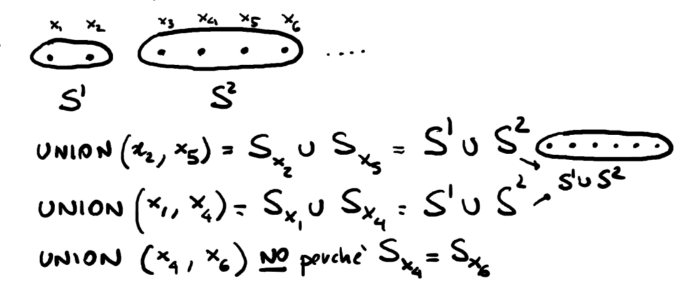
\includegraphics[scale=0.5]{Immagini/Screenshot From 2026-11-16 15-16-21.png}
\end{center}

Il rappresentante di $S_x \cup S_y$ può essere un elemento qualsiasi di $S_x \cup S_y$, di solito si mantiene il rappresentante di $S_x$ (o di $S_y$).

Dopo l'esecuzione di Union($x,y$) la collezione non conterrà più $S_x$ e $S_y$. Al loro posto ci sarà $S_x \cup S_y$

\subsubsection{Post condizioni}
\begin{itemize}
    \item L'esecuzione di una Union riduce di un'unità il numero di insiemi nella collezione $(K \to K-1)$
    \item Partendo da $\{\{x_1\}, \dots, \{x_n\}\}$ dopo $n-1$ Union la collezione diventa $\{X\}$, ossià un insieme contente la collezione di partenza, pertanto un algoritmo che utilizza una struttura dati per insiemi disgiunti \uline{esegue sempre al massimo $n-1$ Union}
\end{itemize}

\subsection{Find-Set: $X \to X$}

$\forall x \in X$, Find-Set($x$) = rapp($S_x$) dove rapp($S_x$) è il rappresentante di $S_x$.

Quindi dato $x \in X$ Find-Set($x$) è il rappresentante (attraverso un puntatore) dell'insieme $S_x$ al quale $x$ appartiene

\begin{center}
    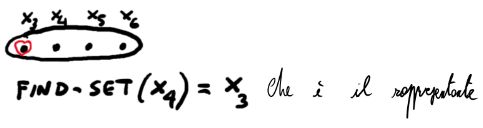
\includegraphics{Immagini/Find-Set.png}
\end{center}

\newpage
\section{Rappresentazione di insiemi disgiunti mediante Liste Concatenate}

\newpage
\section{Rappresentazione di insiemi disgiunti mediante Foreste di insiemi Disgiunti}

\newpage
\section{Calcolo delle componenti connesse di un grafo non orientato}

\subsection{Definizione delle Componenti Connesse}
Una cc di un grafo non orientato $G$ è un sottografo massimale nel quale $\forall i,j$ vertici in cc $j$ è raggiungibile da $i$ ossia è una classe di equivalenza della relazione "raggiungibile"

\subsection{Istanza}
Un sottografo nel quale per ogni coppia di vertici c'è un cammino

\begin{figure}[htbp]
\centering
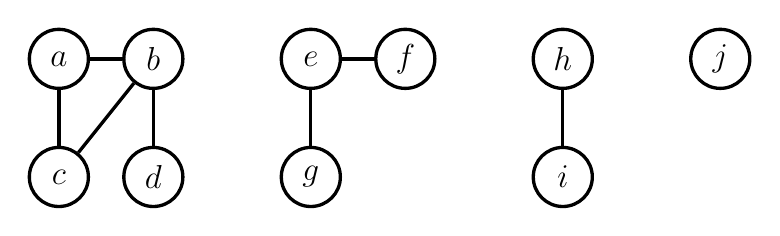
\begin{tikzpicture}[
    vnode/.style={circle, draw=black, very thick, minimum size=7.5mm, inner sep=0pt, font=\large},
    edge/.style={very thick}
]

    % --- 1° Componente Connessa ---
    \node[vnode] (a) at (0, 1.5) {$a$};
    \node[vnode] (b) at (1.2, 1.5) {$b$};
    \node[vnode] (c) at (0, 0) {$c$};
    \node[vnode] (d) at (1.2, 0) {$d$};
    
    \draw[edge] (a) -- (b);
    \draw[edge] (a) -- (c);
    \draw[edge] (b) -- (c);
    \draw[edge] (b) -- (d);

    % --- 2° Componente Connessa ---
    \node[vnode] (e) at (3.2, 1.5) {$e$};
    \node[vnode] (f) at (4.4, 1.5) {$f$};
    \node[vnode] (g) at (3.2, 0) {$g$};
    
    \draw[edge] (e) -- (f);
    \draw[edge] (e) -- (g);

    % --- 3° Componente Connessa ---
    \node[vnode] (h) at (6.4, 1.5) {$h$};
    \node[vnode] (i) at (6.4, 0) {$i$};
    
    \draw[edge] (h) -- (i);

    % --- 4° Componente Connessa ---
    \node[vnode] (j) at (8.4, 1.5) {$j$};

\end{tikzpicture}
\end{figure}

\subsection{Obiettivo}
Calcolare le cc di un grafo.

Si hanno 2 opzioni per fare ciò

\subsection{Soluzione mediante modifica dell'algoritmo DFS}
\begin{minipage}{0.45\textwidth}
    \begin{algorithmic}
        \Procedure{CC-DFS}{$G$}
            \For{ogni $v \in V$}
                \State $v.col=WHITE$
            \EndFor

            \State $k=0$

            \For{ogni $v \in V$}
                \If{$v.col=WHITE$}
                    \State $k=k+1$
                    \State \Call{CC-DFS-VISIT}{$v$}
                \EndIf
            \EndFor
        \EndProcedure
    \end{algorithmic}
\end{minipage}
\hfill
\begin{minipage}{0.45\textwidth}
    \begin{algorithmic}
        \Procedure{CC-DFS-VISIT}{$v$}
            \State $\boxed{v.cc = k}$
            \State $v.col = \text{GRAY}$
            \State $\vdots$
            \For{ogni $v \dots$}
                \State $\vdots$
                \State \Call{CC-DFS-VISIT}{$v$}
            \EndFor
        \EndProcedure
    \end{algorithmic}
\end{minipage}

\subsection{Soluzione sfruttando le strutture dati per insiemi disgiunti con $\mathbf{X=V}$}

Si parte dalla collezione $\{\{v_1\},\{v_2\}, \dots, \{v_n\}\}$ e si vuole arrivare a $\{C^1, \dots, C^n\}$ ove $C^i$ contiene i vertici della cc $i$

\begin{figure}[htbp]
\centering
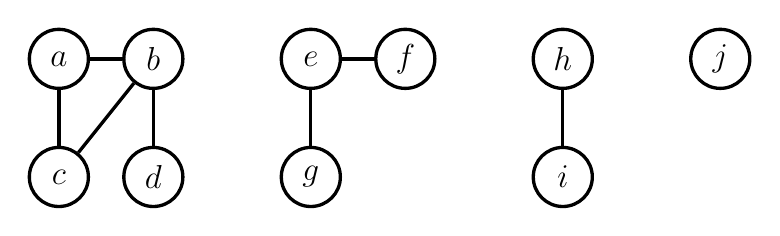
\begin{tikzpicture}[
    vnode/.style={circle, draw=black, very thick, minimum size=7.5mm, inner sep=0pt, font=\large},
    edge/.style={very thick}
]

    % --- 1° Componente Connessa ---
    \node[vnode] (a) at (0, 1.5) {$a$};
    \node[vnode] (b) at (1.2, 1.5) {$b$};
    \node[vnode] (c) at (0, 0) {$c$};
    \node[vnode] (d) at (1.2, 0) {$d$};
    
    \draw[edge] (a) -- (b);
    \draw[edge] (a) -- (c);
    \draw[edge] (b) -- (c);
    \draw[edge] (b) -- (d);

    % --- 2° Componente Connessa ---
    \node[vnode] (e) at (3.2, 1.5) {$e$};
    \node[vnode] (f) at (4.4, 1.5) {$f$};
    \node[vnode] (g) at (3.2, 0) {$g$};
    
    \draw[edge] (e) -- (f);
    \draw[edge] (e) -- (g);

    % --- 3° Componente Connessa ---
    \node[vnode] (h) at (6.4, 1.5) {$h$};
    \node[vnode] (i) at (6.4, 0) {$i$};
    
    \draw[edge] (h) -- (i);

    % --- 4° Componente Connessa ---
    \node[vnode] (j) at (8.4, 1.5) {$j$};

\end{tikzpicture}
\end{figure}

\vspace{0.5cm}

\noindent Nell'esempio si parte da
\[
\Bigl\{ \{a\}, \{b\}, \{c\}, \{d\}, \{e\}, \{f\}, \{g\}, \{h\}, \{i\}, \{j\} \Bigr\}
\]
e si vuole arrivare a
\[
\Bigl\{ \{a, b, c, d\}, \{e, f, g\}, \{h, i\}, \{j\} \Bigr\}
\]
\normalsize

Si uniscono due insiemi disgiunti se $\exists u,v \in V :$
\begin{itemize}
    \item $u \in$ primo insieme
    \item $v \in$ secondo insieme
    \item $(u,v) \in E$
\end{itemize}

si considerano tutti gli archi

{
    \large

    \begin{figure}[htbp]
        \centering

        % --- PARTE 1: Disegno dei grafi (Stato finale) ---
        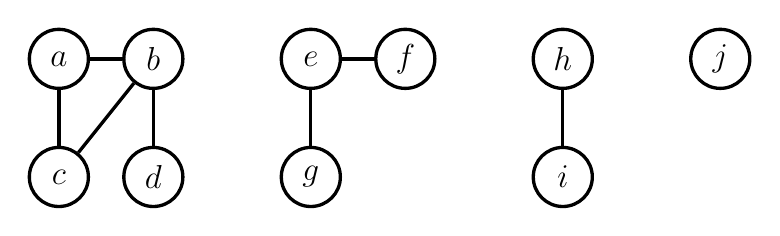
\begin{tikzpicture}[
            vnode/.style={circle, draw=black, very thick, minimum size=7.5mm, inner sep=0pt, font=\large},
            edge/.style={very thick}
        ]

            % Componente 1
            \node[vnode] (a) at (0, 1.5) {$a$};
            \node[vnode] (b) at (1.2, 1.5) {$b$};
            \node[vnode] (c) at (0, 0) {$c$};
            \node[vnode] (d) at (1.2, 0) {$d$};
            \draw[edge] (a) -- (b);
            \draw[edge] (a) -- (c);
            \draw[edge] (b) -- (c);
            \draw[edge] (b) -- (d);

            % Componente 2
            \node[vnode] (e) at (3.2, 1.5) {$e$};
            \node[vnode] (f) at (4.4, 1.5) {$f$};
            \node[vnode] (g) at (3.2, 0) {$g$};
            \draw[edge] (e) -- (f);
            \draw[edge] (e) -- (g);

            % Componente 3
            \node[vnode] (h) at (6.4, 1.5) {$h$};
            \node[vnode] (i) at (6.4, 0) {$i$};
            \draw[edge] (h) -- (i);

            % Componente 4
            \node[vnode] (j) at (8.4, 1.5) {$j$};

        \end{tikzpicture}

        % --- PARTE 2: Tabella di tracciamento operazioni UNION ---
        % Definisco un comando inline per creare la freccia curva con il testo
        \newcommand{\unionarrow}[1]{%
            \begin{tikzpicture}[baseline=-0.7ex]
                \draw[-{Stealth[length=2.5mm]}, thick] (-0.3, 0.5) to[out=0, in=90] (-0.05, 0.25) to[out=-90, in=180] (0.2, 0) node[right, inner sep=2pt, font=\normalsize\bfseries] {UNION (#1)};
            \end{tikzpicture}%
        }

        \[
        \renewcommand{\arraystretch}{1.5} % Aumenta l'altezza delle righe per far respirare le frecce
        \begin{array}{r|l@{\hspace{0.5cm}}l}
            & \{a\} \ \{b\} \ \{c\} \ \{d\} \ \{e\} \ \{f\} \ \{g\} \ \{h\} \ \{i\} \ \{j\} & \\
        \hline
        (b,d) & \{a\} \ \{b,d\} \ \{c\} \ \{e\} \ \{f\} \ \{g\} \ \{h\} \ \{i\} \ \{j\} & \unionarrow{b,d} \\
        (e,g) & \{a\} \ \{b,d\} \ \{c\} \ \{e,g\} \ \{f\} \ \{h\} \ \{i\} \ \{j\}       & \unionarrow{e,g} \\
        (a,c) & \{a,c\} \ \{b,d\} \ \{e,g\} \ \{f\} \ \{h\} \ \{i\} \ \{j\}             & \unionarrow{a,c} \\
        (h,i) & \{a,c\} \ \{b,d\} \ \{e,g\} \ \{f\} \ \{h,i\} \ \{j\}                   & \unionarrow{h,i} \\
        (a,b) & \{a,b,c,d\} \ \{e,g\} \ \{f\} \ \{h,i\} \ \{j\}                         & \unionarrow{a,b} \\
        (e,f) & \{a,b,c,d\} \ \{e,f,g\} \ \{h,i\} \ \{j\}                               & \unionarrow{e,f} \\
        (b,c) & \hspace{1cm} '' \hspace{1.3cm} '' \hspace{1.1cm} '' \hspace{1.1cm} ''   & \quad \textbf{NO UNION} \\
        \end{array}
        \]

    \end{figure}
}

\begin{minipage}{0.45\textwidth}
    \begin{algorithmic}
    \Procedure{CONNECTED-COMPONENT}{$G$}
        \State $G=(V,E)$
        \State $n = |V|$

        \For{$i=1$ to $n$}
            \State \Call{MAKE-SET}{$v_i$}
        \EndFor

        \For{ogni $(u,v) \in E$}
            \If{\Call{FIND-SET}{$u$} $\not = $ \Call{FIND-SET}{$v$}}
                \State \Call{UNION}{$u,v$}
            \EndIf
        \EndFor
    \EndProcedure
\end{algorithmic}
\end{minipage}
\hfill
\begin{minipage}{0.45\textwidth}
    \begin{algorithmic}
        \Procedure{SAME-CC}{$u,v$}
            \If{\Call{FIND-SET}{$u$} = \Call{FIND-SET}{$v$}}
                \State \Return $true$

                \Else
                    \State \Return $false$
            \EndIf
        \EndProcedure
    \end{algorithmic}
\end{minipage}